%By Maria/
 \subsubsection{Pims Login}
Pims Send Notification is a two part function that we tested. First check if user is found(exists) in the database. Then send email using smtp.The unit test codes bellow demonstrates.
\newline

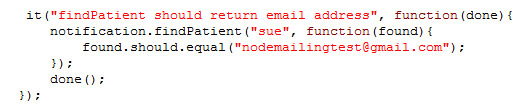
\includegraphics[width=\linewidth]{./Graphics/find.jpg}
\newline

Send Notifications via email
\newline

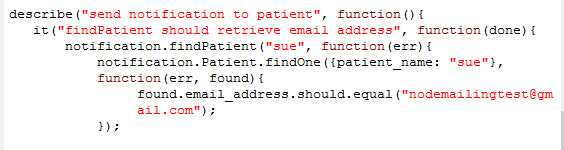
\includegraphics[width=\linewidth]{./Graphics/send.jpg}
The following conditions must be true for the send notification use case to pass.					
	\begin{itemize}
				\item Find patient should query the database to see if a user exists by searching for an email adress.
				\item Oce user is found, send notification must send and email to the found adress.
 \end{itemize}
 
 The figure bellow depics the successful testing of the Send Notification and FindUser functions.
 \newline
 
 \includegraphics[width=\linewidth]{./Graphics/Notify.jpg}
 
 \subsubsection{Remarks}
 	\begin{itemize}
 				\item Pre-Conditions
 		User must exist in database and have and email.
 				\item Post-Conditions
	User recieves and email from Prof Snyman.
  \end{itemize}
  
  Both Pre and Post conditions  are considered in the implimentation of sending notifications. Unit testing successfuly.  tested with no violations to the security of the systm.
 